% !TeX spellcheck = en_US

\documentclass{../UTNetLab}

\title{A Single Segment Network}
\newcommand\reference{
   S. Panwar, S. Mao, J.-dong Ryoo, and Y. Li, “A single segment network,” in TCP/IP Essentials: A Lab-Based Approach, Cambridge: Cambridge University Press, 2004, pp. 43–60.
}

\begin{document}
\part{Network Interface Exercises}
    The following exercises use the single segment network topology shown in \hyperref[fig:1.3]{Figure~1.3}.
    \begin{center}
        \begin{minipage}{0.48\textwidth}
            \begin{flushleft}
                \begin{table}[H]
                    \caption{The IP addresses of the hosts (Table~1.2)}
                    \centering
                    \begin{tabular}{ c c c }
                        \hline \hline
                        Host & IP Address & Subnet Mask \\
                        \hline 
                        h0 & 128.238.66.100 & 255.255.255.0 \\
                        h1 & 128.238.66.101 & 255.255.255.0 \\
                        h2 & 128.238.66.102 & 255.255.255.0 \\
                        h3 & 128.238.66.103 & 255.255.255.0 \\
                        h4 & 128.238.66.104 & 255.255.255.0 \\
                        h5 & 128.238.66.105 & 255.255.255.0 \\
                        h6 & 128.238.66.106 & 255.255.255.0 \\
                        h7 & 128.238.66.107 & 255.255.255.0 \\
                        \hline \hline
                        \end{tabular}
                \end{table}
            \end{flushleft}
        \end{minipage}
        \begin{minipage}{0.48\textwidth}
            \begin{flushright}
                \begin{figure}[H]
                    \centering
                    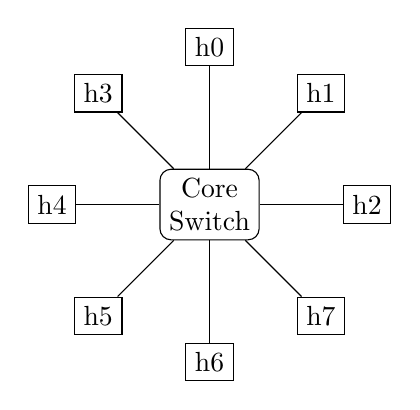
\begin{tikzpicture}
                        \node[draw,align=center,rounded corners] (s) at (0,0){Core\\Switch};
                        \node[draw] (h0) at (0,2){h0};
                        \node[draw] (h1) at ({sqrt(2)},{sqrt(2)}){h1};
                        \node[draw] (h2) at (2,0){h2};
                        \node[draw] (h3) at (-{sqrt(2)},{sqrt(2)}){h3};
                        \node[draw] (h4) at (-2,0){h4};
                        \node[draw] (h5) at (-{sqrt(2)},-{sqrt(2)}){h5};
                        \node[draw] (h6) at (0,-2){h6};
                        \node[draw] (h7) at ({sqrt(2)},-{sqrt(2)}){h7};
                    
                        \draw (h0) -- (s);
                        \draw (h1) -- (s);
                        \draw (h2) -- (s);
                        \draw (h3) -- (s);
                        \draw (h4) -- (s);
                        \draw (h5) -- (s);
                        \draw (h6) -- (s);
                        \draw (h7) -- (s);
                    \end{tikzpicture}
                    \caption{A single segment network (Figure~1.3)}\label{fig:1.3}
                \end{figure}
            \end{flushright}
        \end{minipage}
    \end{center}

\section{Network Interfaces}
    Use the \lstinline{ifconfig -a} command to display information about the network interfaces on the \textit{h0}.
    Find the IP address and the net mask of your machine.
    
    \begin{report}
        \item How many interfaces does the host have?
            List all the interfaces found, give their names, and explain their functions briefly.

        \item What are the MTUs of the interfaces on the \textit{h0}?

        \item Is network subnetted?
            What is the reasoning for your answer? What the experimental are the reasons for subnetting?
    \end{report}


\section{Local Host Dump}
    While \lstinline[emph={lo}]{tcpdump -i lo}\footnote{In old linux use \lstinline[emph={your-host}]{tcpdump host your-host}} is running in one command window, run \lstinline{ping 127.0.0.1} from another command window.

    \begin{report}
        \item From the \lstinline{ping} output, is the 127.0.0.1 interface on?
            Can you see any ICMP message sent from your host in the \lstinline{tcpdump} output?
            Why?
    \end{report}


\section{Network Statistics}
    By using \lstinline{netstat -ie}\footnote{You can use \lstinline{ifconfig} instead.} command, collect the statistics from all the hosts on the network.
    Since we use the same login name and password, we can \lstinline{telnet} to other hosts and run \lstinline{netstat -ie} there.\footnote{%
    After you are done with a remote host, you should exit the \lstinline{telnet} session before you \lstinline{telnet} to another remote host.
    Recursive \lstinline{telnet} will generate unnecessary data in the \lstinline{tcpdump} output and cause confusion.
    }

    Save the \lstinline{netstat -ie} outputs.

    If you don’t see a significant amount of output packets in the \lstinline{netstat} output, the machine was probably restarted recently.
    You may do this experiment later, or use the following \lstinline{socket} command to generate some network traffic:
    \begin{lstlisting}[emph={remote-host},morekeywords={[3]echo}]
# replace remote-host with ip address
socket -u -i -n200 remote-host echo
    \end{lstlisting}
    
    \begin{report}
        \item Calculate the average collision rate over all the hosts for the set of statistics you collected in this exercise.
    \end{report}

\part{ARP Exercises}
    In the following experiment, we shall examine the host ARP table and the ARP operation, including two interesting cases: proxy ARP and gratuitous ARP.
    You may need to find \textbf{MAC} addresses of the host and router interfaces, and record these \textbf{MAC} addresses.
    You need these \textbf{MAC} addresses for the exercises and lab report (as table of host and \textbf{MAC}).

\section{ARP Table}
    Use \lstinline{arp -a} to see the entire ARP table on the \textit{h0}.
    Observe that all the IP addresses displayed are on the same subnet.

    If you find that all the remote hosts are in the \textit{h0}’s ARP table, you need to delete a remote host from the table, using:
    \footnote{If you deleted \textit{h0}’s IP address from the ARP table by mistake, you must add the entry back in the table.
    See the \lstinline{arp} manual page to add.
    Note that, in order for the \textit{h0} to reply to the ARP requests, the ARP entry of \textit{h0} must have the \lstinline{P} flag in the ARP table.}
    \begin{lstlisting}[emph={remote-host}]
arp -d remote-host
    \end{lstlisting}

    Save the ARP table for your lab report.
    
    While \lstinline{tcpdump -en}\footnote{You can add \lstinline{-x} flag to see hex dump.} is running, \lstinline{ping} a remote host that has no entry in the \textit{h0} ARP table.
    Then terminate the \lstinline{tcpdump} program.

    You can run \lstinline{wireshark} to capture network packet by \textbf{start capture} in GNS3 link menu.

    Observe the first few lines of the packet trace to see how ARP is used to resolve an IP address.

    Run \lstinline{arp -a} to see a new line added in the \textit{h0}’s ARP table.
    Save the new ARP table for your lab report.

    Mark the ARP request packet and the ARP reply packet in the \lstinline{wireshark} window.
    Then go to menu \textit{File/Print\ldots} to print the marked packets for your lab report (See Exercise~6 of Chapter~1 of reference book).

    \begin{report}
        \item From the saved \lstinline{tcpdump} output, explain how ARP operates.
            Draw the format of a captured, ARP request and reply including each field and the value.
    \end{report}

    Your report should include the answers for the following questions.
    \begin{itemize}
        \item What is the target IP address in the ARP request?
        \item At the \textbf{MAC} layer, what is the destination Ethernet address of the frame carrying the ARP request?
        \item What is the \texttt{frame} type field in the Ethernet frame?
        \item Who sends the ARP reply?
    \end{itemize}

\section{ARP Timeout}
    While \lstinline[emph={h0,netlab}]{tcpdump host h0.netlab} is running to capture traffic from the \textit{h0} machine, execute \lstinline{telnet 128.238.66.200}.
    Note there is no host with this IP address in the current configuration of the lab network.

    Save the \lstinline{tcpdump} output of the first few packets for the lab report.

    After getting the necessary output, terminate the \lstinline{telnet} session.

    \begin{report}
        \item From the saved \lstinline{tcpdump} output, describe how the ARP timeout and retransmission were performed.
            How many attemps were made to resolve a non-existing IP address?
    \end{report}

\section{ARP Proxy}
    The network topology for this proxy ARP exercise is shown in \hyperref[fig:2.9]{Figure~2.9}.
    The IP addresses and network masks for the hosts are also given in \hyperref[fig:2.9]{Figure~2.9}.
    Change the IP address and network mask of \textit{h0} accordingly (see Section~2.3.2 of reference book).
    Change the IP addresses and network masks of the \textit{Router4} interfaces according to \hyperref[fig:2.9]{Figure~2.9}.

    \textbf{Note}\quad
    Network mask of the hosts in the 128.238.65.0 network is 255.255.0.0.
    
    \textbf{Note}\quad
    Only use \textit{h0, h1, h4, h5} hosts (Do not start extra hosts).

    Set IP of each network by running the following command in the hosts:
    \begin{enumerate}
        \item \lstinline[emph={x,eth0},morekeywords={[3]masks}]{ifconfig eth0 x.x.x.x/mask}
        \item \lstinline[emph={y},morekeywords={[3]add,default,gw}]{route add default gw y.y.y.y}
    \end{enumerate}
    Next we will enable the proxy ARP function on the ethernet1 interface of \textit{Router4}.
    \begin{enumerate}
        \item \lstinline{telnet} to \textit{Router4}.
                (Right click on the Router and open console on GNS3 or use \lstinline{telnet 128.238.64.4}.)
        \item Log in to the router, type \lstinline[language={cisco}]{enable} to enter the \textit{Privileged EXEC} mode.\footnote{We will discuss bridge and router configuration in Chapter~3.}
        \item Enter the \textit{Global Configuration} mode by typing \lstinline[language={cisco}]{config term}.
        \item Then type the following lines for each interfaces:
        \begin{lstlisting}[language={cisco}, escapechar={@}, emph={x}]
! config term
    interface f0/0 ! use f0/1 for the other interface@\footnote{The name of the router interfaces may be different for various routers.
    You can find the names by typing \texttt{write term} in the \textit{Privilege EXEC} mode.}@
        ip addr x.x.x.x 255.255.255.0
        no shut
        ip proxy-arp
        Ctrl-Z
wr
        \end{lstlisting}
    \end{enumerate}
    
    Now \textit{Router4}’s \textit{ethernet1} interface can perform proxy ARP for the hosts in the 128.238.64.0 subnet.

    Run \lstinline{tcpdump -enx} on the \textit{h1} and the \textit{h5}.

    Then let the hosts in the 128.238.65.0 subnet send UDP datagrams to the hosts in the 128.238.64.0 subnet.
    For example, on the \textit{h4} type:
    \begin{lstlisting}[emph={host-in-64-0-subnet},morekeywords={[3]echo}]
socket -i -u -n1 -w1000 host-in-64-0-subnet echo
    \end{lstlisting}

    When you are done with all the hosts in the 128.238.64.0 subnet, save the \lstinline{tcpdump} output for the lab report.

    Run \lstinline{arp -a} to display the new ARP table in the \textit{h1}, \textit{h4} and the \textit{h5}.
    Save the ARP table for your lab report.

    % After the lab instructor restores the network into a single subnet (see \hyperref[fig:1.3]{Figure~1.3}), change the IP address and network mask of your host’s interface back to their default values as in \hyperref[fig:1.3]{Figure~1.3}.

    \begin{figure}[H]
        \centering
            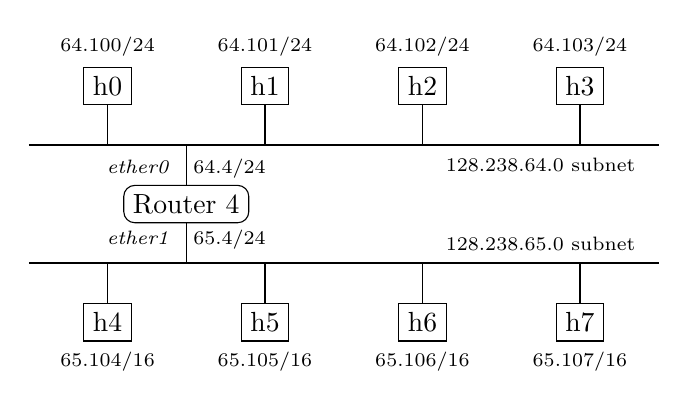
\begin{tikzpicture}
                \draw (0*2,3) node[draw,fill=white] (h0) {h0} -- +(0,-0.75) +(0,+0.5) node {\scriptsize 64.100/24};
                \draw (1*2,3) node[draw,fill=white] (h1) {h1} -- +(0,-0.75) +(0,+0.5) node {\scriptsize 64.101/24};
                \draw (2*2,3) node[draw,fill=white] (h2) {h2} -- +(0,-0.75) +(0,+0.5) node {\scriptsize 64.102/24};
                \draw (3*2,3) node[draw,fill=white] (h3) {h3} -- +(0,-0.75) +(0,+0.5) node {\scriptsize 64.103/24};
                \draw (0*2,0) node[draw,fill=white] (h4) {h4} -- +(0,+0.75) +(0,-0.5) node {\scriptsize 65.104/16};
                \draw (1*2,0) node[draw,fill=white] (h5) {h5} -- +(0,+0.75) +(0,-0.5) node {\scriptsize 65.105/16};
                \draw (2*2,0) node[draw,fill=white] (h6) {h6} -- +(0,+0.75) +(0,-0.5) node {\scriptsize 65.106/16};
                \draw (3*2,0) node[draw,fill=white] (h7) {h7} -- +(0,+0.75) +(0,-0.5) node {\scriptsize 65.107/16};
                \draw (0.5*2,1.5) node[draw,rounded corners,fill=white] (r4) {Router 4}
                    -- +(0,+0.75) +(0,+0.45) node {\scriptsize\textit{ether0}\quad 64.4/24}
                    -- +(0,-0.75) +(0,-0.45) node {\scriptsize\textit{ether1}\quad 65.4/24}
                ;
                \draw[thick] (-1,0.75) -- +({(3+1)*2},0);
                \draw[thick] (-1,2.25) -- +({(3+1)*2},0);
                \node at ({-1+(3+0.25)*2},2) {\scriptsize 128.238.64.0 subnet};
                \node at ({-1+(3+0.25)*2},1) {\scriptsize 128.238.65.0 subnet};
            \end{tikzpicture}
        \caption{Network configuration (Figure~2.9)}\label{fig:2.9}
    \end{figure}
    
    \begin{report}
        \item Explain the operation of proxy ARP.

        \item Why can a host in the 128.238.65.0 subnet reach a host in the 128.238.64.0 subnet, even though they have different subnet IDs?

        \item What are the \textbf{MAC} addresses corresponding to hosts in the 128.238.64.0 subnet, in the ARP table of a host in the 128.238.65.0 subnet?

        \item Give one advantage and one disadvantage of using proxy ARP.
    \end{report}

\section{** Gratuitous (Unsolicited) ARP}
    While \lstinline{tcpdump -ex} (or run \lstinline{wireshark}) is running on all the hosts, reboot host \textit{h7}.
    You can send the gratuitous ARP manually by execute:

    \begin{lstlisting}[emph={eth0,h7-ip,h6-ip}]
arping -c 4 -A -I eth0 h6-ip
arping -c 4 -U -I eth0 h7-ip
    \end{lstlisting}

    After \textit{h7} is started, terminate \lstinline{tcpdump} and run \lstinline{wireshark -r exe7.out &} to load the \lstinline{tcpdump} trace.
    Print the gratuitous ARP request for your lab report.
    
    \begin{report}
        \item What is the purpose of gratuitous ARP?
    
        \item List the sender IP address, target IP address, sender \textbf{MAC} address, and target \textbf{MAC} address of the gratuitous ARP you saved.

        \item What is the ARP table in the \textit{h5}?
    \end{report}


\part{Exercise with ICMP and \texttt{ping}}\label{sec:icmp-ping}
    The following exercises use the previous network topology shown in \hyperref[fig:2.9]{Figure~2.9}.

\section{ping ICMP}
    Use \lstinline[emph={h1,netlab}]{ping -sv h1.netlab} on the \textit{h0} to test whether the \textit{h1} host is reachable, while running:\\
    \lstinline[emph={h0,h1,netlab},morekeywords={[3]host,and}]{tcpdump -enx host h0.netlab and h1.netlab}.
    Save the \lstinline{tcpdump} and \lstinline{ping} output for the future study on \lstinline{ping}.
    
    \begin{report}
        \item What ICMP messages are used by \lstinline{ping}?
    \end{report}

\section{ICMP Port Unreachable}
    While running \lstinline[emph={h0,h1,netlab}]{tcpdump -x -s 70 host h0.netlab and h1.netlab}, execute the following \lstinline{socket} command to send a UDP datagram to the \textit{h1} host from the \textit{h0}:

    \begin{lstlisting}[emph={h0,h1,netlab}]
socket -i -u -n1 -w1000 h1.netlab 88888
    \end{lstlisting}

    Save the \lstinline{tcpdump} output for the lab report.

    \begin{report}
        \item Study the saved ICMP port unreachable error message (See \hyperref[fig:2.7]{Figure~2.7} of reference book.).
            Why are the first 8 bytes of the original IP datagram payload included in the ICMP message?
    \end{report}

\section{ICMP Host Unreachable}
    While \lstinline{tcpdump} is running to capture the ICMP messages, \lstinline{ping} a host with IP address \textbf{128.238.60.100} on \text{h2}.
    Save the \lstinline{ping} output.
    
    \begin{report}
        \item Can you see any traffic sent on the network? Why? Explain what happened from the \lstinline{ping} output.

        \item List the different ICMP messages you captured in \nameref{sec:icmp-ping}.
            Give the values of the type and code fields.
    \end{report}

\part{Exercises with IP address and subnet mask}
    In this section, we will observe what happens when the same IP address is assigned to two different hosts.
    We will also set an incorrect subnet mask for hosts and see what are the consequences.
    For the next two exercises, we use only four host from single segment network (\hyperref[fig:1.3]{Figure~1.3}).

\section{Duplicate IP}\label{sec:duplicate-ip}
    Change the IP address of your hosts as shown in \hyperref[tab:2.3]{Table~2.3}.

    \begin{table}[H]
        \caption{Host IP addresses and network masks for \nameref{sec:duplicate-ip} (Table~2.3)}\label{tab:2.3}
        \centering
        \begin{tabular}{ c c c c }
            \hline \hline
            Host & IP Address & Subnet Mask \\
            \hline 
            h0 & 128.238.66.100 & 255.255.255.0 \\
            h1 & 128.238.66.100 & 255.255.255.0 \\
            h2 & 128.238.66.102 & 255.255.255.0 \\
            h3 & 128.238.66.103 & 255.255.255.0 \\
            \hline \hline
            \end{tabular}
    \end{table}

    Delete the entries for all hosts other than your host from ARP table.

    Run \lstinline{tcpdump -enx} on all the hosts.
    Then, do the following three experiments:

    \begin{enumerate}
        \item Execute \lstinline{telnet} from one of two hosts with the duplicate IP address to a host with unique IP address (e.g.\ \textit{h0} $\rightarrow$ \textit{h2}).

        Now, from the other host with the duplicate IP address, execute \lstinline{telnet} command to the same host (\textit{h1} $\rightarrow$ \textit{h2}).

        Observe what happens and save the \lstinline{tcpdump} output and the ARP tables in all the hosts in your group.
        
        \item Execute \lstinline{telnet 128.238.66.100} (or \lstinline{telnet 128.238.66.104}) from the \textit{h2}.
        Which host provides the telnet connection?
        Why?
        
        \item Execute \lstinline{telnet 128.238.66.100} (or \lstinline{telnet 128.238.66.104}) from the \textit{h3}.
    Which host is connected to \textit{h3}? Why?
    \end{enumerate}
    
    \begin{report}
        \item Explain what happened in the first case and why.
            Answer the questions for the second and third cases.
    \end{report}

    \newpage

\section{IP Subnets}\label{sec:ip-subnets}
    Change the host IP addresses and the subnet masks as shown in \hyperref[tab:2.4]{Table~2.4}.
    Note that two hosts in each group (\textit{h0} and the \textit{h3}) are assigned an incorrect subnet mask.

    \begin{table}[H]
        \caption{Host IP addresses and network masks for \nameref{sec:ip-subnets} (Table~2.4)}\label{tab:2.4}
        \centering
        \begin{tabular}{ c c c }
            \hline \hline
            Host & IP Address & \makebox[7.3em][c]{Subnet Mask} \\
            \hline 
            h0 & 128.238.66.100 & \makebox[7.3em][l]{255.255.255.240} \\
            h1 & 128.238.66.101 & \makebox[7.3em][l]{255.255.255.0} \\
            h2 & 128.238.66.102 & \makebox[7.3em][l]{255.255.255.0} \\
            h3 & 128.238.66.120 & \makebox[7.3em][l]{255.255.255.240} \\
            \hline \hline
            \end{tabular}
    \end{table}

    Capture the packets with \lstinline{tcpdump -e} for the following cases.

    \begin{enumerate}
        \item When \textit{h0} \lstinline{ping}s one of the hosts that have the correct subnet mask.
        
        \item When \textit{h3} \lstinline{ping}s one of the hosts that have the correct subnet mask.

        Now, copy the output displayed from the \lstinline{ping} window in the \textit{h3}.
        Share the saved output message with other students.
        
        \item When a host with the correct subnet mask \lstinline{ping}s \textit{h0}.
        
        \item When a host with the correct subnet mask \lstinline{ping}s \textit{h3}.
    \end{enumerate}
    
    To avoid confusion, only one machine in each group should generate traffic in each case.
    Clearly, this exercise has to be performed as a team.
    
    \begin{report}
        \item Explain what happened in each case according to the \lstinline{tcpdump} outputs saved.
            Explain why \textit{h3} could not be reached from other hosts, whereas \textit{h0}), which has the same incorrect subnet mask, could communicate with the other hosts.
    \end{report}
\end{document}
